%%%%%%%%%%%%%%%%%%%%%%%%%%%%%%%%%%%%%%%%%
% TU Muenchen 17 Sommer Semester 
% Applied Reinforcement Learning
% 1st Report 
%%%%%%%%%%%%%%%%%%%%%%%%%%%%%%%%%%%%%%%%%

%----------------------------------------------------------------------------------------
%	PACKAGES AND OTHER DOCUMENT CONFIGURATIONS
%----------------------------------------------------------------------------------------

\documentclass[
11pt, % Main document font size
a4paper, % Paper type, use 'letterpaper' for US Letter paper
oneside, % One page layout (no page indentation)
%twoside, % Two page layout (page indentation for binding and different headers)
headinclude%footinclude, % Extra spacing for the header and footer
BCOR3mm, % Binding correction
]{scrartcl}

%%%%%%%%%%%%%%%%%%%%%%%%%%%%%%%%%%%%%%%%%
% Arsclassica Article
% Structure Specification File
%
% This file has been downloaded from:
% http://www.LaTeXTemplates.com
%
% Original author:
% Lorenzo Pantieri (http://www.lorenzopantieri.net) with extensive modifications by:
% Vel (vel@latextemplates.com)
%
% License:
% CC BY-NC-SA 3.0 (http://creativecommons.org/licenses/by-nc-sa/3.0/)
%
%%%%%%%%%%%%%%%%%%%%%%%%%%%%%%%%%%%%%%%%%

%----------------------------------------------------------------------------------------
%	REQUIRED PACKAGES
%----------------------------------------------------------------------------------------

\usepackage[
nochapters, % Turn off chapters since this is an article        
beramono, % Use the Bera Mono font for monospaced text (\texttt)
eulermath,% Use the Euler font for mathematics
pdfspacing, % Makes use of pdftex’ letter spacing capabilities via the microtype package
dottedtoc % Dotted lines leading to the page numbers in the table of contents
]{classicthesis} % The layout is based on the Classic Thesis style

\usepackage{arsclassica} % Modifies the Classic Thesis package

\usepackage[T1]{fontenc} % Use 8-bit encoding that has 256 glyphs

\usepackage[utf8]{inputenc} % Required for including letters with accents

\usepackage{graphicx} % Required for including images
\graphicspath{{Figures/}} % Set the default folder for images

\usepackage{enumitem} % Required for manipulating the whitespace between and within lists

\usepackage{lipsum} % Used for inserting dummy 'Lorem ipsum' text into the template

\usepackage{subfig} % Required for creating figures with multiple parts (subfigures)

\usepackage{amsmath,amssymb,amsthm} % For including math equations, theorems, symbols, etc

\usepackage{varioref} % More descriptive referencing

%----------------------------------------------------------------------------------------
%	THEOREM STYLES
%---------------------------------------------------------------------------------------

\theoremstyle{definition} % Define theorem styles here based on the definition style (used for definitions and examples)
\newtheorem{definition}{Definition}

\theoremstyle{plain} % Define theorem styles here based on the plain style (used for theorems, lemmas, propositions)
\newtheorem{theorem}{Theorem}

\theoremstyle{remark} % Define theorem styles here based on the remark style (used for remarks and notes)

%----------------------------------------------------------------------------------------
%	HYPERLINKS
%---------------------------------------------------------------------------------------

\hypersetup{
%draft, % Uncomment to remove all links (useful for printing in black and white)
colorlinks=true, breaklinks=true, bookmarks=true,bookmarksnumbered,
urlcolor=webbrown, linkcolor=RoyalBlue, citecolor=webgreen, % Link colors
pdftitle={}, % PDF title
pdfauthor={\textcopyright}, % PDF Author
pdfsubject={}, % PDF Subject
pdfkeywords={}, % PDF Keywords
pdfcreator={pdfLaTeX}, % PDF Creator
pdfproducer={LaTeX with hyperref and ClassicThesis} % PDF producer
} % Include the structure.tex file which specified the document structure and layout

\hyphenation{Fortran hy-phen-ation} % Specify custom hyphenation points in words with dashes where you would like hyphenation to occur, or alternatively, don't put any dashes in a word to stop hyphenation altogether

%----------------------------------------------------------------------------------------
%	TITLE AND AUTHOR(S)
%----------------------------------------------------------------------------------------

\title{\normalfont\spacedallcaps{Finding the Shortest Path Using Reinforcement Learning}} % The article title
\author{\spacedlowsmallcaps{Lingfeng Zhang, Wenhan Hao, $\&$ Tianming Qiu}} % The article author(s) - author affiliations need to be specified in the AUTHOR AFFILIATIONS block
\date{Group: applied-rl17 / E3} % An optional date to appear under the author(s)

%----------------------------------------------------------------------------------------

\begin{document}

%----------------------------------------------------------------------------------------
%	HEADERS
%----------------------------------------------------------------------------------------

\renewcommand{\sectionmark}[1]{\markright{\spacedlowsmallcaps{#1}}} % The header for all pages (oneside) or for even pages (twoside)
%\renewcommand{\subsectionmark}[1]{\markright{\thesubsection~#1}} % Uncomment when using the twoside option - this modifies the header on odd pages
\lehead{\mbox{\llap{\small\thepage\kern1em\color{halfgray} \vline}\color{halfgray}\hspace{0.5em}\rightmark\hfil}} % The header style

%\pagestyle{scrheadings} % Enable the headers specified in this block

\maketitle % Print the title/author/date block

%----------------------------------------------------------------------------------------
%	INTRODUCTION
%----------------------------------------------------------------------------------------

\section{Introduction}

%A statement\footnote{Example of a footnote} requiring citation \cite{Figueredo:2009dg}.

\quad 
Path planning is a widely-studied and basic problem. 
Also it has many actual scenarios, for example, for autonomous car navigation and drones for logistics. 
Considering about distance and traffic situation, the optimal path between start and destination will be figured out. 
It is related to mathematics, optimal research, and artificial intelligence. 
Although there are already many existing algorithms to find the best path, we shall attempt to solve this problem with reinforcement learning.

This project offers an agent which could find the shortest path between two locations in a unfamiliar road network and thus reduce the cost of time and energy.

%Some mathematics in the text: $\cos\pi=-1$ and $\alpha$.
 
%----------------------------------------------------------------------------------------
%	Project description
%----------------------------------------------------------------------------------------

\section{Project description}

\begin{figure}[tb]
\centering 
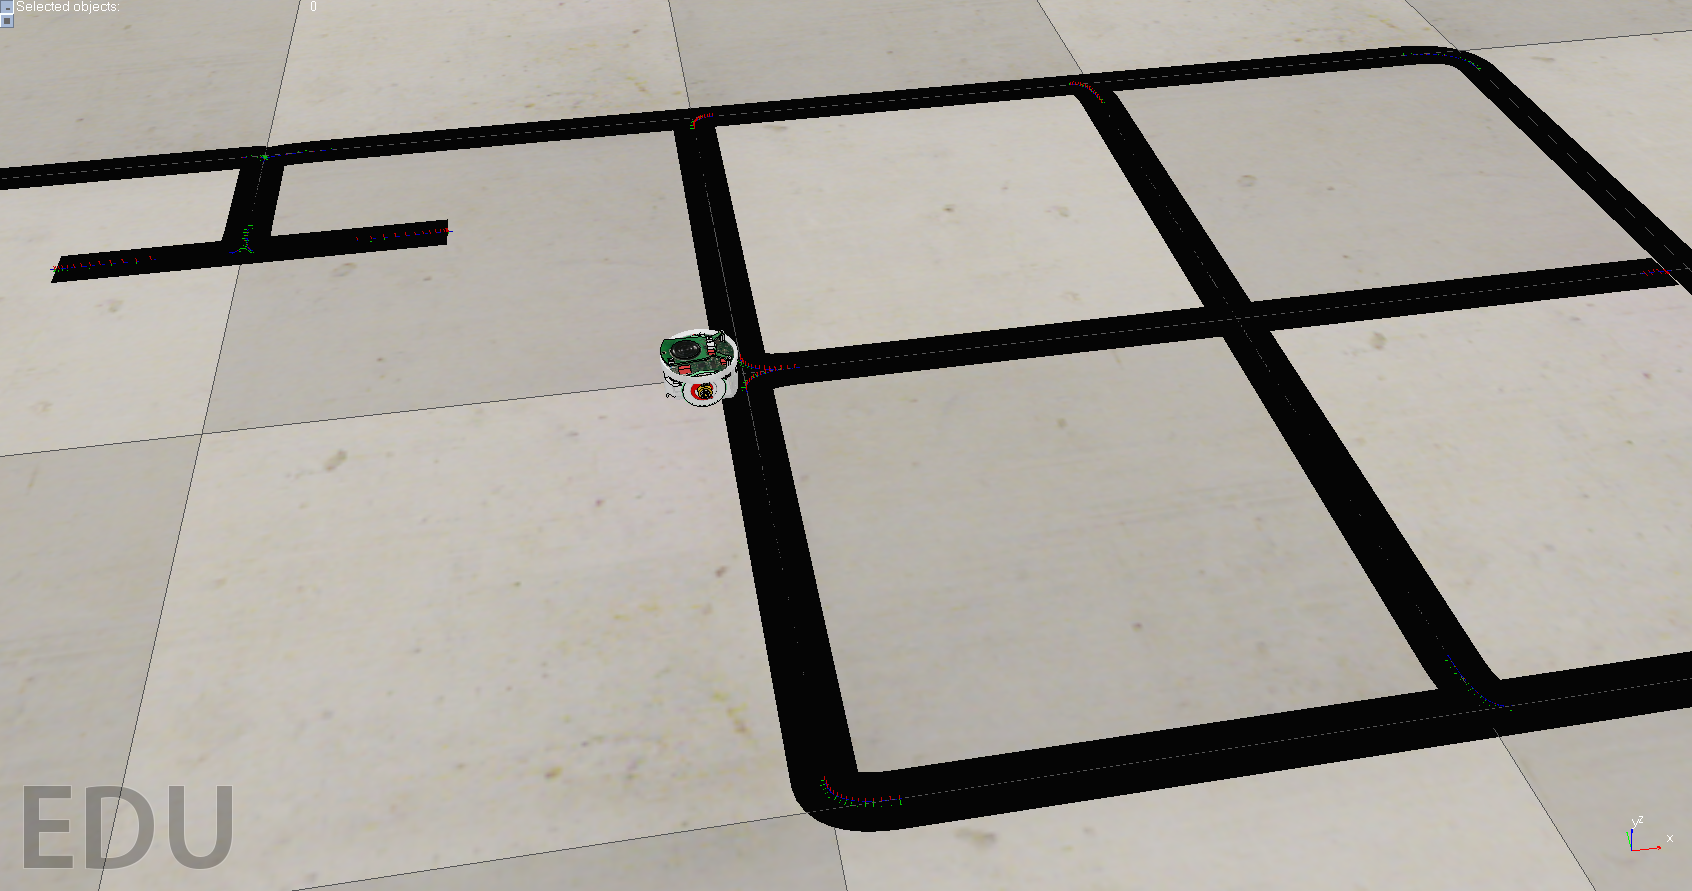
\includegraphics[width=0.5\columnwidth]{simulatemap} 
\caption[An example of a floating figure]{An example of simulate map} % The text in the square bracket is the caption for the list of figures while the text in the curly brackets is the figure caption
\label{fig:gallery} 
\end{figure}

\quad 
Instead of the real road network in a city or a building, 
a simulated network will be adopted, which contains several straight lines on the ground as the roads to form the road network with many crossroads. 
This simulated example map is showed in Figure~\vref{fig:gallery}. % The \vref command specifies the location of the reference.
Arbitrary two points of them could de chose as starting point and destination.

In this project we will use E-puck as the test agent. 
The E-puck robot will be first placed at the starting point and start to explore the road network. 
It will make a decision which direction it should go at every crossroad. Once the E-puck reach the destination, 
it will be replaced at the same starting point. 
During the learning process, E-pack will take a random direction at each crossroad. 
Every time E-puck arrive at the destination successfully it will update all the value function of each state. After several trials, 
the E-puck may find the shortest path to the destination according the latest value functions.



%----------------------------------------------------------------------------------------
%	3.	Model
%----------------------------------------------------------------------------------------

\section{Model}

\quad The model part includes how we disgn the states, actions, reward and value function as well as how the algorithm works.

%------------------------------------------------

\subsection{State}
\quad
In this project, we will consider different crossroads in the simulated map as the states. 
A preliminary conception would include a road network with 8-10 states. 
We are aware of difficulties in recognizing the different states.
In addition, the obstacles will be not considered as states. 
And in the simulated map we will also set some blind alleys, they can be treated as states but with very poor rewards.

After brainstorming, we have two tentative solution for this problem:


First, a concept of ‘photoelectric encoder’ would be adopted. 
We will draw some specific patterns, for example like black-and-white stripes unit, at the crossroads. And we could use the under sensor on E-puck to scan the patterns to determine the current state. 


Alternative we could use the front CMOS color camera to recognize the different street signs we put at the crossroads in order to determine the states. 
On the street signs we decided to write the capital letter such as just ‘A’, ‘B’, ‘C’ and so on. 
Then we use some computer vision techniques such as feature detection and matching to recognize which pattern the image is. 
Afterwards the E-puck can understand at which crossroads it is.


Since the image transforming and processing is so computation-assuming that E-puck cannot handle with properly even make the E-puck to halt. 
So we consider about combination of two solutions. 
That means we will set some specific patterns on the road ground especially before the crossroad to let the E-puck know it is approaching the crossroad and ready to start the program of image processing. 
Then E-puck could wait for few seconds at crossroad to judge and make correct decisions during learning process.

%----------------------------------
\subsection{Action}
The actions for E-puck would be not difficult. We adopt just ‘turn right’, ‘’turn left’, ‘go straight’ and ‘backward’ naively. 


In details, for the ‘backward’ action we will not accept the method that directly make the wheel rotate inversely to go backward because the E-peck is designed to detect the states always by using its front CMOS color camera. 
Therefore we ought to design a safe solution to make E-puck turn round and change into the opposite direction and make sure that it would be still in the middle of the road. Unless it would be a little trouble for following activities.

%-------------------------------------
\subsection{Reward}
Reward setting is always the most difficult part in reinforcement learning algorithm. 
In this model we will assign a reward ‘+10’ at the destination state and ‘0’ at the other states. 
Also at the ‘blind alley’ it will get a very poor reward such as ‘-100’.



%-----------------------------------
\subsection{Q function}
\quad
We decide to use \textsl{Q-Learning}(Watkins, 1989), defined by
\begin{equation}
\mathit{Q(S_t,A_t)\xleftarrow{}  Q(S_t,A_t)+ }\alpha \mathit{[ R_{t+1} + }\gamma \mathit{\max \limits_{a}Q(S_{t+1},a)-Q(S_t,A_t)]}
\end{equation}
\quad And an off-policy TD control algorithm would be adopted.
At each iteration step the Q function would be updated and the action would be taken greedily.



%----------------------------------------------------------------------------------------
%	Project management
%----------------------------------------------------------------------------------------
\section{Project management}

\paragraph{Stage 1} familiar with Python and Vrep simulation environment

\paragraph{Stage 2} according the primary conception, 
we will design a simple map with less than 10 states to test and modify both the modeling and algorithm

\paragraph{Stage 3} confirm the modeling, optimize our algorithm
\paragraph{Stage 4} tranfrom the program from simulation environment to the real E-puck





\end{document}